\chapter{実験1}
\section{データセット \label{sec:ch2:dataset}}
実験に用いるデータセットとして,
IMDB-wikiデータセット
\cite{Rothe-ICCVW-2015,Rothe-IJCV-2018,imdb-wiki}を用いた.
このデータセットは(主に海外の)映画やドラマの
情報をまとめているオンラインデータベースであるIMDbと
オンラインの百科事典であるWikipediaに含まれる顔写真を
人名や性別,年齢などのタグをつけてデータセット化したものである.
今回の作成するシステムは,入力対象の顔写真を
男性に限定している.そこで,性別情報の含まれるデータセットを利用した.

IMDB-wikiデータセットは自動的にWeb上の情報から
各画像にタグをつけているため,そのタグが必ずしも
正確であるとは限らない.また,
Wikipediaのデータに関しては一部に破損がある問題も存在する.

そのため,今回の実験ではIMDbのデータのみを利用することにし,
そのデータをさらにクリーニングすることにした.
IMDbに含まれる顔写真は主に女優・俳優のものになる.

データのクリーニングは以下の手段で実行した.
\begin{enumerate}
  \item 性別タグが男性であるものを抽出する
  \item IMDb-wikiに含まれる,AIによる顔検出スコアの上位2000件を抽出する.
  \item 名前情報を用いて,同一人物の写真を顔検出スコアが最も高いもの以外削除する.
  \item 目視による手動作業で,タグミスによる女性の写真,複数人が
  写っているもの,白黒写真を除外した.
\end{enumerate}
結果,1076件の異なる男性の顔カラー写真が抽出できた.

\section{クラウドソーシングの実施}
IMDB-wikiデータセットから抽出した顔写真に対して,
クラウドソージングによってワーカーに印象(impression)ラベルを
付与していただき,実験に用いるデータセットとする.

クラウドソージングにはAmazon Mechanical Turk (AMT,mTurk)を利用した.
これは,IMDbが主に海外の映画・ドラマを対象にしていることや,
システムで用いる7つの印象が英語の印象(impression)であることを考慮し,
主にアメリカ人がワーカーとして活動している
\footnote{
2010年の研究では
ワーカーの57\%がアメリカ人,32\%がインド人であると
報告されている\cite{10.1145/1753846.1753873}.
現在はその比率も大きく変化しているとも考えられ,
AMTのワーカーが主にアメリカ人であると仮定するのは
誤っている可能性も高い.
}AMTを利用することが最適であると
考えたためである.

\subsection{タスクインストラクション}
AMTを用いて,画像に対して複数の印象を選択する
クラウドソージングタスクを作成した.
図\ref{fig:ch2:task}にタスクのスクリーンショットを示す.
\begin{figure}[tb]
  \centering
  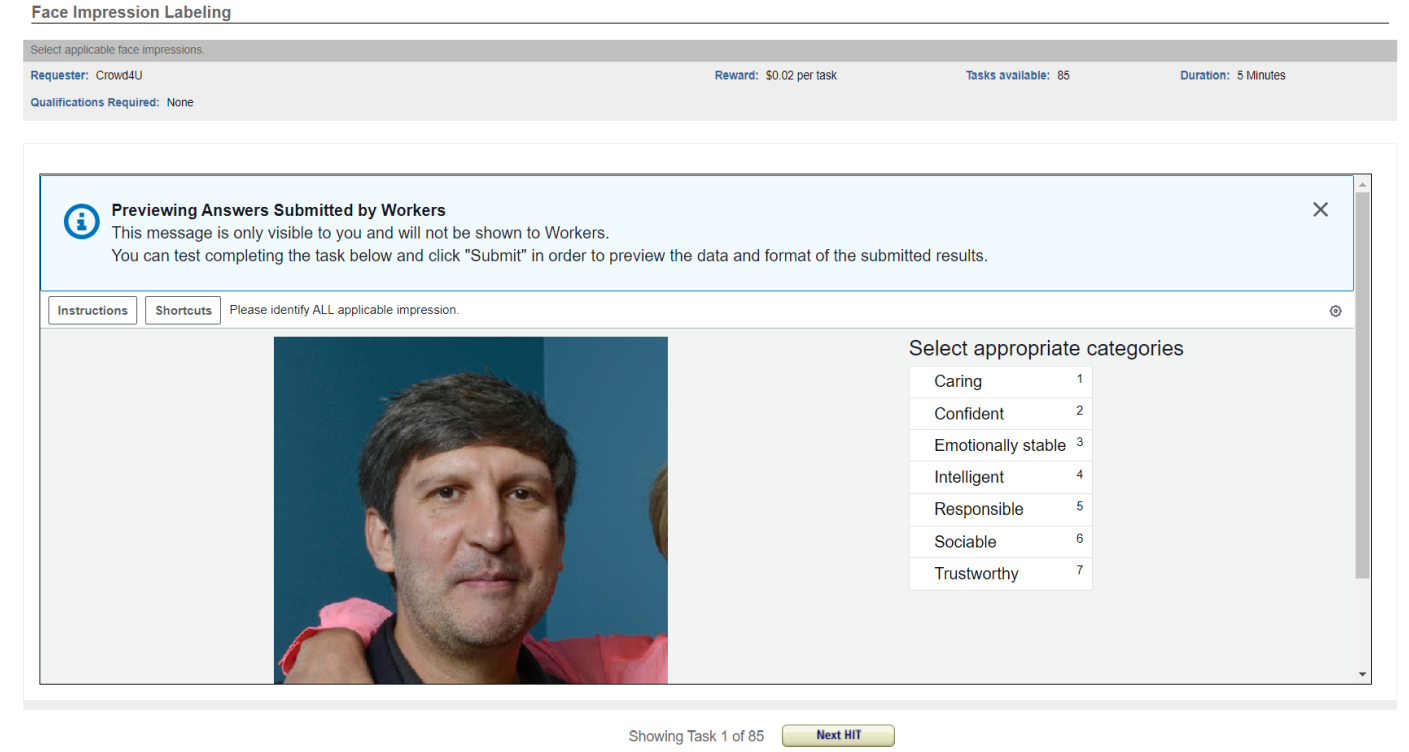
\includegraphics[width=12cm]{ch2/task.png}
  \caption{
  クラウドソージングタスクのスクリーンショット
  \label{fig:ch2:task}
  }
\end{figure}
タスクの説明などは以下のように設定した.
\begin{itemize}
  \item Project Name: Face Impression Labeling
  \item Title: Select applicable face impressions.
  \item Description: Please identify ALL applicable
  face impression labels with the given photo.
  You can select multi labels each photo, if you
  think several labels match the face.
  \item Keywords: categorize, image
\end{itemize}

AMTでは画像に対して複数のタグを選択させる場合,
crowd-image-classifier-multi-selectを用いることができる.

\subsection{人数・値段・工夫した点}
以下のように人数・値段を設定した.
\begin{itemize}
  \item 1タスク3ワーカー
  \item 1タスク当たりのワーカー報酬は\$0.02
  \item 1タスク当たりのAMT手数料は\$0.01
  \item 85タスク実施
\end{itemize}
よって
請求金額は,
85タスク$\times$3ワーカー$\times$\$0.03$=$\$7.65となった.
タスク数85は1000円という予算を考慮して決定した数である.
1タスクあたり3秒と見積もっており,
時給換算すると\$24となる.これは
インフレを考慮しても,アメリカの最低賃金
を大幅に上回る額であると考えられる.

\ref{sec:ch2:dataset}節で抽出した顔写真のうち,
顔検出スコアの高い85枚を抽出し,
筑波大学全学計算機システムWeb公開サービスを用いて
タスクに埋め込んだ.

クラウドソージングタスクを作成するのは初めてだったので,
勉強を兼ねて,1タスクあたりのワーカー数を3に設定し,
結果の多数決による統合などを試してみることにした.
3は多数決を行える最も小さい数値である.

誤って男性とタグ付けされている写真を削除するなど.
あらかじめデータセットをクリーニングしておいたことで,
無意味なタスクを実行してしまう可能性を下げることが
できたと考えられる.これはクラウドソーシングを
行う上で工夫した点の一つである.

\section{クラウドソーシングの結果}
\section{機械学習の実施}
\section{機械学習の結果}